\documentclass[twocolumn,12pt,a4paper]{article}
\usepackage[latin1]{inputenc}
\usepackage[T1]{fontenc} 
\usepackage[english]{babel} 

\pagestyle{empty} 

\usepackage{graphicx}
\usepackage{amsmath, amsthm}
\newtheorem{theorem}{Theorem}
\newtheorem{proposition}{Proposition}
\newtheorem{lemma}{Lemma}
\newtheorem*{proof*}{Proof}
\newtheorem{definition}{Definition}

\newtheorem{exercise}{Exercise}
\newtheorem{question}{Question}

\newtheorem{example}{Example}

\newtheorem{remark}{Remark}

\usepackage[a4paper,left=.8cm, right=.8cm,top=1.5cm,bottom=1.5cm]{geometry}
\setlength{\columnsep}{1.2cm}

\usepackage{cancel}
\usepackage{bm}
\usepackage{amssymb,amsfonts}
\usepackage{mathrsfs}
\usepackage{color}
%\usepackage{hyperref}
\usepackage{dsfont}
\usepackage{graphicx}
\usepackage{algorithmicx}
\usepackage[ruled]{algorithm}
\usepackage{algpseudocode}
\usepackage{marginnote}
\newcommand{\Ptr}{\mathcal P^{\rm tr}}
\newcommand{\tr}{{\rm tr}}
\newcommand{\N}{\mathbb N}
\newcommand{\calN}{\mathcal N}
\newcommand{\bP}{\bold P}
\newcommand{\calK}{\mathcal K}
\newcommand{\calF}{\mathcal F}
\newcommand{\calH}{\mathcal H}
\newcommand{\calP}{\mathcal P}
\newcommand{\calC}{\mathcal C}
\newcommand\red[1]{\textcolor{red} {#1} }
\newcommand{\R}{\mathbb R}
\newcommand{\bX}{\bar X}
\newcommand{\Ktr}{\calK^{\rm tr}}
\title{ \bfseries \Huge {Handout 3: Discrete-time Markov chains (1) }}    
\vspace{-4cm}        

\date{Due date : March $24^{th}$}       
\vspace{-4cm}        
\newcounter{num}  % Create a new counter for paragraphs
\begin{document}
	\maketitle
	\setcounter{num}{1}  % Start the paragraph counter at 1
	
	\thispagestyle{empty} 
	\paragraph{Brief recap:}
	
	
	\paragraph{Exercise \thenum.}
	Consider a continuous-time Markov chain \( X(t) \) that has the jump chain shown in Figure 11.26 (this is the same Markov chain given in Example 11.19). Assume \( \lambda_1 = 2 \), \( \lambda_2 = 1 \), and \( \lambda_3 = 3 \).
	\vspace{-.5cm}  
		\begin{figure}[h!]
		\begin{center}
		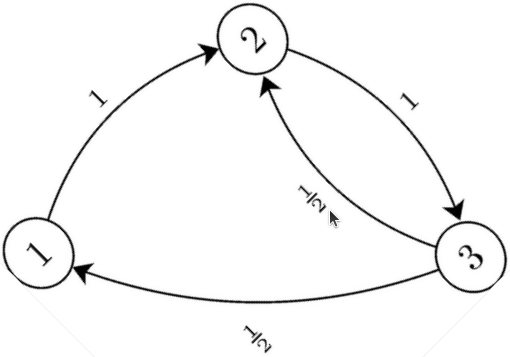
\includegraphics[width = .3\textwidth]{images/ctmc_1.png}
		\end{center}
	\end{figure}
	\vspace{-1cm}        
	\begin{enumerate}
		\item Find the generator matrix for this chain.
		\item Find the limiting distribution for \( X(t) \) by solving \( \pi G = 0 \).
	\end{enumerate}
	
	
	\stepcounter{num} 
	\paragraph{Exercise \thenum.}
	Suppose that customers arrive according to a Poisson process with rate \( \lambda \) at a service center that has a single server. Customers are served one at a time in order of arrival. Service times are assumed to be i.i.d. Exponential(\( \mu \)) random variables and independent of the arrival process. Customers leave the system after being served. Our goal in this problem is to model the above system as a continuous-time Markov chain. Let \( X(t) \) be the number of customers in the system at time \( t \), so the state space is \( S = \{0, 1, 2, \dots\} \). Assume \( i > 0 \). If the system is in state \( i \) at time \( t \), then the next state would either be \( i + 1 \) (if a new customer arrives) or state \( i - 1 \) (if a customer leaves).
	
	\begin{enumerate}
		\item Suppose that the system is in state 0, so there are no customers in the system and the next transition will be to state 1. Let \( T_0 \) be the time until the next transition. Show that \( T_0 \sim \text{Exponential}(\lambda) \).
		
		\item Suppose that the system is currently in state \( i \), where \( i > 0 \). Let \( T_i \) be the time until the next transition. Show that \( T_i \sim \text{Exponential}(\lambda + \mu) \).
		
		\item Suppose that the system is at state \( i \). Find the probability that the next transition will be to state \( i + 1 \).
		
		\item Draw the jump chain, and provide the holding time parameters \( \lambda_i \).
		
		\item Find the Generator matrix.
		
		\item Draw the transition rate diagram.
	\end{enumerate}
	
	
	\stepcounter{num} 
	\paragraph{Exercise \thenum.}
	
	
	\stepcounter{num} 
	\paragraph{Exercise \thenum.}
	
	
	\stepcounter{num} 
	\paragraph{Exercise \thenum.}
	
	
%	https://www.probabilitycourse.com/chapter11/11_3_4_solved_probs.php
\end{document}